\section{Scans}

CT scans are a reconstruction of the measurements collected during the scanning process. With their help, we can 'slice up the body' and look at what is inside in a non-invasive way. Slices are represented as a matrix called reconstruction matrix. These matrices consist of voxels - three-dimensional boxes. 

In \ref{fig:ct-brain-slices} you can see a number of axial (in the direction parallel to the body) slices of the human brain: 

\begin{figure}[ht]
    \centering
    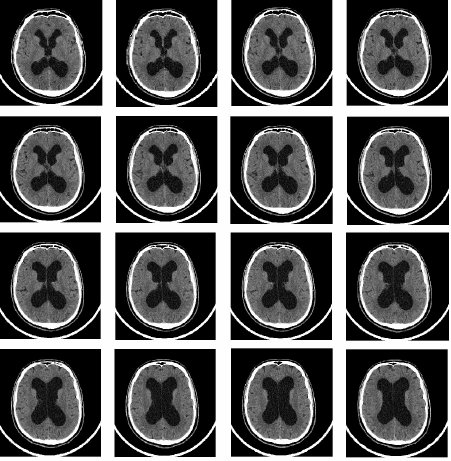
\includegraphics[width=200pt]{images/ct-brain-slices.jpg}
    \caption[CT brain slices]{CT brain slices \cite{brain-image}}
    \label{fig:ct-brain-slices}
\end{figure}

During the reconstruction phase, attenuation value for every voxel in the slice is assigned. Attenuation refers to loss of intensity of the ray passing through the tissue. These values can be computed by using simple algorithms like ART or Backprojection.

The attenuation values for every voxel are then transformed into Hounsfield units using this formula:

\begin{equation}
    \mathrm{CT number = [K \times (u_{voxel}-u_{water})]/u_{water}}
\end{equation}

\textit{K} is a constant nowadays set for 1000. \textit{$u_{voxel}$} and \textit{$u_{water}$} correspond to selected voxel's attenuation and water's attenuation respectively. This formula implies attenuation of water is 0 and the range of CT number is between -1000 and 1000. However, when it comes to images, we usually work with 256 greyscale values and the CT numbers need to be normalised. \cite{goldman2007}

\subsection{Artifacts}
CT scans are prone to artifacts. The reason for this is that a CT scan is computed from thousands of measurements. Any error in a measurement or computation of the voxel attenuation can be propagated to the image as an artifact. Basically, artifacts are attenuation values which do not correspond to the attenuation of the original tissue.

There are many ways in which an artifact can occur. Some of them stem from an incorrect position of the patient's body, physical processes occurring during data gathering or errors from reconstructing CT data. Artifacts can manifest themselves as streaks, shading, rings or distortion. They can be suppressed either on the side of CT manufacturers or by the operator \cite{barrett-keat2004}.  

\subsection{Formats}
There are two popular formats for storing CT and other medical images - DICOM and NIfTI. DICOM is a standard format scanners usually export the data in, whereas NIfTI is a more light-weighted format DICOM is typically converted to. 

DICOM is very complex and robust. With the introduction of CT, there was a need for ``a standard method for transferring images and associated information between devices manufactured by various vendors'' \cite{DICOM-spec}. Every object in the file is encapsulated in a tag. Objects store various types of information, for example data about the patient or the actual image data. Objects contain a tag (a two-number code, which defines the purpose of the object), VR (information about the data type), length of the data and in the end, the data itself \cite{neuro2016}.

NIfTI was firstly developed for use in neuroscience and with fMRI images specifically. The goal was to create a tool, that would be available for the whole research community, easy to use and suitable for a wide range of applications. NIfTI format is able to store not only data sets, but also for example statistical data. NIfTI files consist of a header and the actual data, either together in one .nii file, or separatly as .hdr and .img (header and image respectively) files. The header is 348 bytes long and its fields contain information about dimensionality, data type or data scaling. \cite{nifti} 

\subsection{Orientation}
When talking about medical images, it is important to know vocabulary related to directions. There are three axis describing 6 directions (Fig. \ref{fig:orientations}. Right and Left on the right-left axis correspond to the right and left directions. Anterior means towards front, posterior towards back. Inferior means below, towards the feet and superior means towards the head.

\begin{figure}[ht!]
    \centering
    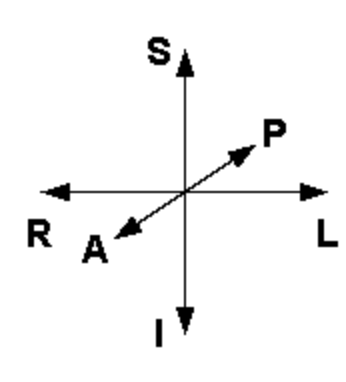
\includegraphics[width=150pt]{images/orientation.png}
    \caption[Orientations]{R - left to RIGHT, L - right to LEFT, A - posterior to ANTERIOR, P - anterior to POSTERIOR, I - superior to INFERIOR, S - inferior to SUPERIOR}
    \label{fig:orientations}
\end{figure}

Two popular coordinate systems are RAS and LAS. That means the first axis points to right (or left respectively), the second to anterior and the third to superior. RAS is a system used by neurologists and LAS by radiologists. 

We usually work with two spaces: scanner (world) space and voxel space. For the scanner space, the origin of the coordinate system is at the magnet isocentre. For voxel space, the origin is in the centre of the first voxel in the array. For example, if voxels are organised as RAS, it means voxels in rows are stored from left to right. Rows are stored from posterior to arterior to create a slice. And slices are ordered from inferior to superior to produce the whole image volume. It is possible to ``switch'' between these spaces using affine transformation. \cite{coordinate-systems}